\documentclass[12pt,a4paper]{amsart}
% ukazi za delo s slovenscino -- izberi kodiranje, ki ti ustreza
\usepackage[slovene]{babel}
%\usepackage[cp1250]{inputenc}
%\usepackage[T1]{fontenc}
\usepackage[utf8]{inputenc}
\usepackage{amsmath,amssymb,amsfonts}
\usepackage{url}
%\usepackage[normalem]{ulem}
\usepackage[dvipsnames,usenames]{color}
\usepackage{graphicx}

% ne spreminjaj podatkov, ki vplivajo na obliko strani
\textwidth 15cm
\textheight 24cm
\oddsidemargin.5cm
\evensidemargin.5cm
\topmargin-5mm
\addtolength{\footskip}{10pt}
\pagestyle{plain}
\overfullrule=15pt % oznaci predlogo vrstico


% ukazi za matematicna okolja
\theoremstyle{definition} % tekst napisan pokoncno
\newtheorem{definicija}{Definicija}[section]
\newtheorem{primer}[definicija]{Primer}
\newtheorem{opomba}[definicija]{Opomba}

\renewcommand\endprimer{\hfill$\diamondsuit$}


\theoremstyle{plain} % tekst napisan posevno
\newtheorem{lema}[definicija]{Lema}
\newtheorem{izrek}[definicija]{Izrek}
\newtheorem{trditev}[definicija]{Trditev}
\newtheorem{posledica}[definicija]{Posledica}


% za stevilske mnozice uporabi naslednje simbole
\newcommand{\R}{\mathbb R}
\newcommand{\N}{\mathbb N}
\newcommand{\Z}{\mathbb Z}
\newcommand{\C}{\mathbb C}
\newcommand{\Q}{\mathbb Q}


% ukaz za slovarsko geslo
\newlength{\odstavek}
\setlength{\odstavek}{\parindent}
\newcommand{\geslo}[2]{\noindent\textbf{#1}\hspace*{3mm}\hangindent=\parindent\hangafter=1 #2}


% naslednje ukaze ustrezno popravi
\newcommand{\program}{Finančna matematika} % ime studijskega programa
\newcommand{\imeavtorja}{Katarina Brilej, Sara Kovačič} % ime avtorja
\newcommand{\imementorja}{prof.~dr. Riste Škrekovski} % akademski naziv in ime mentorja
\newcommand{\naslovdela}{Uporaba metahevristike GRASP na problemu potujočega trgovca}
\newcommand{\letnica}{2019} %letnica 


% vstavi svoje definicije ...




\begin{document}

% od tod do povzetka ne spreminjaj nicesar
\thispagestyle{empty}
\noindent{\large
UNIVERZA V LJUBLJANI\\[1mm]
FAKULTETA ZA MATEMATIKO IN FIZIKO\\[5mm]
\program\ -- 1.~stopnja}
\vfill

\begin{center}{\large
\imeavtorja\\[2mm]
{\bf \naslovdela}\\[10mm]
Projekt OR pri predmetu Finančni praktikum\\[1cm]
Mentor: \imementorja}
\end{center}
\vfill

\noindent{\large
Ljubljana, \letnica}
\pagebreak

\thispagestyle{empty}
%%%%     \tableofcontents PRI KRATKEM POROČILU NI SMISELNO KAZALO - dodaj pri dolgem
\pagebreak



% tu se zacne besedilo seminarja
\section{Uvod}


Metahevristika je algoritemski način reševanja kombinatoričnega optimizacijskega problema, pri katerem na začetku izberemo množico kandidatov za rešitev, in jo iterativno izboljšujemo (glede na neko vnaprej izbrano funkcijo zaželenosti), ter po dovolj korakih vrnemo najboljši element iz te množice. Metahevristike torej vrnejo približne rešitve, a veliko hitreje kot eksaktni postopki. V projektu bova na problem potujočega trgovca implementirali metahevristiko GRASP (\textit{greedy randomized adaptive search procedure}). Problem potujočega trgovca bova rešili tudi kot celoštevilski linearni program in primerjali rešitve. Generirali bova nekaj zanimivih grafov in na njih preizkusili algoritem. Rezultate bova primerjail tudi z rezultati iz spleta in rezultati skupine 7, ki bo na problem potujočega trgovca implementirala genetski algoritem. 


\section{Problem potujočega trgovca} 

Problem potujočega trgovca (”travelling salesman problem”/TSP) se glasi:


\begin{itemize}
\item {\bf Formulacija v vsakdanjem jeziku:} danih je $n$ mest in razdalja med poljubnim parom mest (od mesta do mesta lahko potujemo po zgolj eni poti). Najdi najkrajšo (najcenejšo) pot, ki se začne in konča v istem mestu ter obišče vsako mesto natanko enkrat.
\item{\bf Formulacija v matematičnem jeziku}: v (neusmerjenem enostavnem) polnem grafu $K_n$ z uteženimi povezavami (pozitivne vrednosti) najdi najkrajši cikel, ki vsebuje vsa vozlišča. Ciklom, ki vsebujejo vsa vozlišča grafa, pravimo Hamiltonovi cikli.

\end{itemize}
\hfill \break

\subsection{Celoštevilski linearni program in primerjava z GRASP}  \hfill \break


Problem potujočega trgovca lahko predstavimo kot \textit{celoštevilski linearni program}.
Označimo mesta s števili $1, \ldots, n$. Strošek (ali razdalja) potovanja iz mesta $i$ v mesto $j$ je $c_{i,j}$, ( $ 1\leq i, j\leq n$). Minimiziramo strošek potovanja. Definiramo:

$$ X_{i,j} := \left\{ \begin{array}{ll}
1 ~; & \textrm{potnik gre iz mesta $i$ v mesto $j$}, \\
0 ~; & \textrm{sicer},
\end{array} \right. $$

\hfill \break

$y_{i}$ \ldots katero po vrsti obiščemo mesto $i$


\begin{equation*}
\begin{aligned}
& {\text{min}}
& & \sum_{i=1}^{n} \sum_{j=1}^{n}  x_{i,j} \cdot c_{i,j} \\
& \text{p. p.}
& &\sum_{i=1}^{n} x_{i,j} = 1, \text{ za vsak $j$ }\\
&&&\sum_{j=1}^{n} x_{i,j} = 1, \text{ za vsak $i$ }\\
&&&  x_{i,j} \in \{0,1\}, \text{ za vsak $i$ in vsak $j$ }\\
&&& y_{i} \in \{1, \ldots, n\}; \text{za vsak $i$}\\
&&& y_{i} + 1 - n + n \cdot x_{i,j} \leq y_{j}; \text{za vsak $i$ in vsak $j>1$}
\end{aligned}
\end{equation*}

Problem potujočega trgovca se da v pythonu elegantno zapisati kot celoštevilski linearni program s pomočjo knjižnice PuLP. PuLP za reševanje problema izbere enega od vgrajenih algoritmov. V našem primeru je PuLP za reševanje izbral PULP\_CBC\_CMD. S pomočjo knjižnice PuLP sva napisali funckijo, ki sprejme matriko cen povezav, izpiše minimalno ceno potovanja in vrne urejen seznam obiskanih mest. 
Z merjenjem časa reševanja določenih primerov različnih velikosti ugotovimo, da napisana funkcija $ilp$ porabi več časa za reševanje, kot metahevristika $GRASP$. 

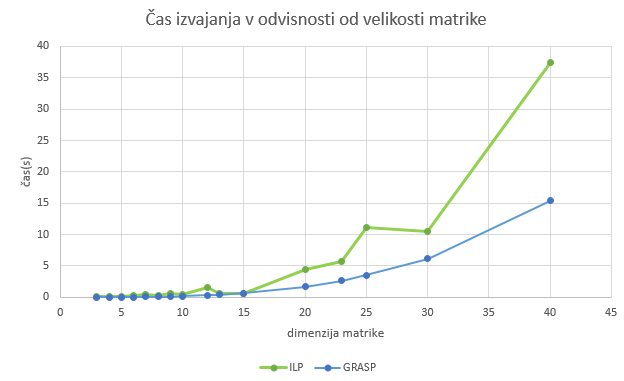
\includegraphics[scale =0.8]{casilp}

\section{Grasp} 

GRASP (\textit{greedy randomized adaptive search procedure}) je metahevristika, ki sestoji iz dveh faz: \textit{greedy randomized construction} in \textit{local search}.
V prvi fazi na pameten način (odvisno od problema) izberemo izmed vseh možnih rešitev CL (candidate list) množico začetnih približkov RCL (restricted candidates list). 
To storimo deloma deterministično in deloma stohastično, da zagotovimo, da so začetni približki obetavni, a dovolj razpršeni po celotni množici CL, da bo druga faza pregledala čimvečji del CL. 
V drugi fazi za vsako izmed teh rešitev$ s \in  RCL $ pregledamo elemente $s' \in CL$ v njeni okolici (kaj je okolica je od problema in načina reševanja odvisno). Če najdemo boljšo rešitev $s'$, 
jo dodamo v RCL ter $s$ odstranimo. To ponavljamo dokler zaustavitveni pogoj (npr. št. iteracij, zahtevana natančnost) ni izpolnjen.

\section{Nadaljnje delo}

 

\pagebreak
% seznam uporabljene literature
\begin{thebibliography}{99}

\bibitem{Wikipedia TSP}
Travelling salesman problem
\\\texttt{http://en.wikipedia.org/wiki/Travelling\_salesman\_problem}


\end{thebibliography}

\end{document}

